\begin{pastexam}[label={px:gw3-112-ds-02}]{關務三等資訊處理 112 年 第二題}
（申論；25 分）

用G = (V, E)表示一個無方向性圖形，其中 V 是點的集合，E 是一組節點（Vertices）形成邊的集合。今有一圖形 G = (V, E)，
$V(G)$ = \{T, W, X, Y, Z\}, $E(G)$ = \{(T, W),(T, Y),(T, Z),(W, X),(W, Z),(X, Z)\}，每一個邊對應的權重值分別為 2, 1, 7, 4,
3, 6，請用相鄰矩陣（Adjacency Matrix）與相鄰串列（Adjacency List）表示此圖形，並使用 Prim's 演算法，計算最小成本擴張
樹（Minimum Cost Spanning Tree），依序寫出從點 X 加入邊的順序，最小成本擴張樹的權重總和為何？（25 分）
\end{pastexam}

\begin{pastsoln}
答案：加入邊的順序 (X, W) 4、(W, T) 2、(T, Y) 1、(W, Z) 3；權重總和 $10$。

邊和權重的對應：$(T,W) = 2$、$(T,Y) = 1$、$(T,Z) = 7$、$(W,X) = 4$、$(W,Z) = 3$、$(X,Z) = 6$。
\begin{center}
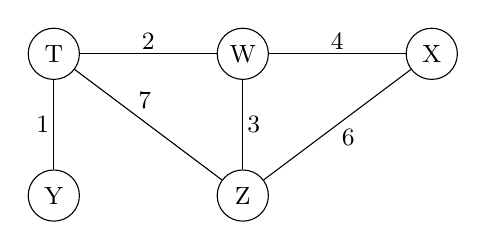
\begin{tikzpicture}[v/.style={circle,draw,minimum size=6.5mm,inner sep=0pt,font=\small},
  w/.style={font=\small,inner sep=1.5pt}]
\node[v] (T) at (0,0) {T};
\node[v] (W) at (2.4,0) {W};
\node[v] (X) at (4.8,0) {X};
\node[v] (Y) at (0,-1.8) {Y};
\node[v] (Z) at (2.4,-1.8) {Z};
\draw (T) -- node[w,above] {2} (W);
\draw (T) -- node[w,left] {1} (Y);
\draw (T) -- node[w,above right,pos=0.4] {7} (Z);
\draw (W) -- node[w,above] {4} (X);
\draw (W) -- node[w,right] {3} (Z);
\draw (X) -- node[w,below right] {6} (Z);
\end{tikzpicture}
\end{center}

\textbf{相鄰矩陣}（資結書第~21.2~節）：頂點依 T, W, X, Y, Z 編號，$a_{ij}$ 是邊 $(i, j)$ 的權重，沒有邊記 $\infty$，
對角線記 $0$。 無向圖的矩陣是對稱的。
\[
\begin{array}{c|ccccc}
 & T & W & X & Y & Z \\ \hline
T & 0 & 2 & \infty & 1 & 7 \\
W & 2 & 0 & 4 & \infty & 3 \\
X & \infty & 4 & 0 & \infty & 6 \\
Y & 1 & \infty & \infty & 0 & \infty \\
Z & 7 & 3 & 6 & \infty & 0
\end{array}
\]

\textbf{相鄰串列}：每個頂點一條串列，節點存「相鄰頂點, 權重」；無向圖每條邊在兩端各出現一次，共 $2 \times 6 = 12$ 個節點。
\begin{center}
\small
\begin{tabular}{ll}
T & $\to$ (W, 2) $\to$ (Y, 1) $\to$ (Z, 7) \\
W & $\to$ (T, 2) $\to$ (X, 4) $\to$ (Z, 3) \\
X & $\to$ (W, 4) $\to$ (Z, 6) \\
Y & $\to$ (T, 1) \\
Z & $\to$ (T, 7) $\to$ (W, 3) $\to$ (X, 6) \\
\end{tabular}
\end{center}

\textbf{Prim 演算法}（資結書第~24.3~節）：從 X 開始，每次在「一端在樹內、一端在樹外」的邊中選權重最小的加入。
\begin{center}
\small
\begin{tabular}{clll}
\toprule
步驟 & 樹內頂點 & 候選邊（權重） & 加入 \\
\midrule
1 & \{X\} & (X,W) 4、(X,Z) 6 & (X, W) 4 \\
2 & \{X, W\} & (W,T) 2、(W,Z) 3、(X,Z) 6 & (W, T) 2 \\
3 & \{X, W, T\} & (T,Y) 1、(W,Z) 3、(X,Z) 6、(T,Z) 7 & (T, Y) 1 \\
4 & \{X, W, T, Y\} & (W,Z) 3、(X,Z) 6、(T,Z) 7 & (W, Z) 3 \\
\bottomrule
\end{tabular}
\end{center}
$5$ 個頂點、$4$ 條邊，樹完成。 加入邊的順序：\textbf{(X, W)、(W, T)、(T, Y)、(W, Z)}，權重總和 $4 + 2 + 1 + 3 = \mathbf{10}$。
\begin{center}
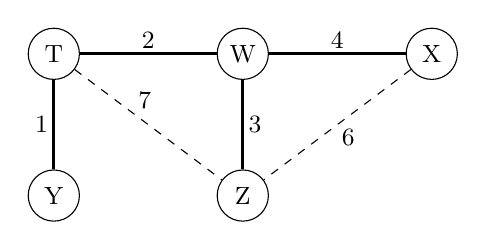
\begin{tikzpicture}[v/.style={circle,draw,minimum size=6.5mm,inner sep=0pt,font=\small},
  w/.style={font=\small,inner sep=1.5pt}]
\node[v] (T) at (0,0) {T};
\node[v] (W) at (2.4,0) {W};
\node[v] (X) at (4.8,0) {X};
\node[v] (Y) at (0,-1.8) {Y};
\node[v] (Z) at (2.4,-1.8) {Z};
\draw[very thick] (T) -- node[w,above] {2} (W);
\draw[very thick] (T) -- node[w,left] {1} (Y);
\draw[dashed] (T) -- node[w,above right,pos=0.4] {7} (Z);
\draw[very thick] (W) -- node[w,above] {4} (X);
\draw[very thick] (W) -- node[w,right] {3} (Z);
\draw[dashed] (X) -- node[w,below right] {6} (Z);
\end{tikzpicture}
\end{center}
（粗線是最小成本擴張樹。）檢查：不在樹上的邊 $(T,Z) = 7$ 和 $(X,Z) = 6$ 各自和樹上的路徑形成環，環上它都是最大的
（$7 > 2, 3$；$6 > 4, 3$），由環性質（資結書定理~24.3）可知這棵樹是最小的；所有權重都不同，所以最小成本擴張樹唯一，
從哪一點出發做 Prim 都得到同一棵，只是加入的順序不同。
\end{pastsoln}
